\documentclass[article]{jss}

\usepackage[utf8]{inputenc}
\usepackage[english]{babel}
\usepackage[document]{ragged2e}
\usepackage{geometry} % see geometry.pdf on how to lay out the page. There's lots.
\usepackage{enumerate}
\usepackage[super]{nth}
\usepackage{graphicx}
\usepackage{hyperref}
\usepackage{amsmath}
\usepackage{ctable}
\usepackage{longtable}
\usepackage{float}
\usepackage{placeins}
\usepackage{Sweave}
\usepackage{mathtools}
\usepackage{array}
\usepackage{tabu}
\usepackage{color, colortbl}
\usepackage{csvsimple}
\usepackage{mathtools}
\usepackage{amssymb}
\usepackage{setspace}
\usepackage{listings}
\usepackage[ruled,vlined]{algorithm2e}
\usepackage{color} %red, green, blue, yellow, cyan, magenta, black, white
\definecolor{mygreen}{RGB}{28,172,0} % color values Red, Green, Blue
\definecolor{mylilas}{RGB}{170,55,241}
\restylefloat{table}
% 
% \DefineVerbatimEnvironment{Sinput}{Verbatim} {xleftmargin=2em,
%                                               frame=single}
% \DefineVerbatimEnvironment{Soutput}{Verbatim}{xleftmargin=2em,
%                                               frame=single}
%                                               
% \DefineVerbatimEnvironment{Sinput}{Verbatim} {xrightmargin=2em,
%                                               frame=single}
% \DefineVerbatimEnvironment{Soutput}{Verbatim}{xrightmargin=2em,
%                
%% -- LaTeX packages and custom commands ---------------------------------------

%% recommended packages
\usepackage{thumbpdf,lmodern}

%% another package (only for this demo article)
\usepackage{framed}


%% new custom commands
\newcommand{\class}[1]{`\code{#1}'}
\newcommand{\fct}[1]{\code{#1()}}

%% For Sweave-based articles about R packages:
%% need no \usepackage{Sweave}



%% -- Article metainformation (author, title, ...) -----------------------------

%% - \author{} with primary affiliation
%% - \Plainauthor{} without affiliations
%% - Separate authors by \And or \AND (in \author) or by comma (in \Plainauthor).
%% - \AND starts a new line, \And does not.
\author{First Author\\ETH Zürich
   \And Second Author\\Plus Affiliation}
\Plainauthor{First Author, Second Author}

%% - \title{} in title case
%% - \Plaintitle{} without LaTeX markup (if any)
%% - \Shorttitle{} with LaTeX markup (if any), used as running title
\title{Vignette Template: The \pkg{goldfish} package in \proglang{R}}
\Plaintitle{Vignette Template: The goldfish package in R}
\Shorttitle{The \pkg{goldfish} package in \proglang{R}}

%% - \Abstract{} almost as usual
\Abstract{
  This short article illustrates how to write a manuscript for the
  \emph{Journal of Statistical Software} (JSS) using its {\LaTeX} style files.
  Generally, we ask to follow JSS's style guide and FAQs precisely. Also,
  it is recommended to keep the {\LaTeX} code as simple as possible,
  i.e., avoid inclusion of packages/commands that are not necessary.
  For outlining the typical structure of a JSS article some brief text snippets
  are employed that have been inspired by \cite{Zeileis+Kleiber+Jackman:2008},
  discussing count data regression in \proglang{R}. Editorial comments and
  instructions are marked by vertical bars.
}

%% - \Keywords{} with LaTeX markup, at least one required
%% - \Plainkeywords{} without LaTeX markup (if necessary)
%% - Should be comma-separated and in sentence case.
\Keywords{JSS, style guide, comma-separated, not capitalized, \proglang{R}}
\Plainkeywords{JSS, style guide, comma-separated, not capitalized, R}

%% - \Address{} of at least one author
%% - May contain multiple affiliations for each author
%%   (in extra lines, separated by \emph{and}\\).
%% - May contain multiple authors for the same affiliation
%%   (in the same first line, separated by comma).
\Address{
  Achim Zeileis\\
  Journal of Statistical Software\\
  \emph{and}\\
  Department of Statistics\\
  Faculty of Economics and Statistics\\
  Universit\"at Innsbruck\\
  Universit\"atsstr.~15\\
  6020 Innsbruck, Austria\\
  E-mail: \email{Achim.Zeileis@R-project.org}\\
  URL: \url{https://eeecon.uibk.ac.at/~zeileis/}
}

\begin{document}
\Sconcordance{concordance:article.tex:article.Rnw:%
1 55 1 1 10 99 1 1 2 4 0 1 2 1 1 1 4 2 1 1 2 4 0 1 2 4 1 %
1 2 13 0 1 2 8 1 1 4 1 2 6 1 1 89 8 1 1 2 9 1 1 3 13 0 1 %
2 4 1 1 2 4 0 1 2 10 1 1 5 6 0 1 2 4 1 1 4 6 0 1 2 33 1 1 %
2 9 1 1 3 15 0 1 2 3 1 1 2 4 0 1 2 10 1 1 3 5 0 1 2 6 1 1 %
5 4 1 1 3 5 0 1 2 6 1 1 14 23 0 1 2 4 1 1 7 1 2 10 1 1 5 %
2 1 1 2 11 0 1 2 2 1 1 4 6 0 1 2 9 1 1 2 4 0 1 2 9 1 1 4 %
6 0 1 2 17 1 1 13 8 1 1 3 5 0 1 2 1 1 1 4 6 0 1 2 8 1 1 4 %
6 0 1 2 10 1 1 3 5 0 1 2 1 1 1 2 11 0 1 2 3 1 1 3 5 0 1 2 %
1 1 1 2 16 0 1 2 189 1}


\justify
\section[Introduction]{Introduction} \label{sec:intro}


Social networks change through time, and researchers from various disciplines have an interest in understanding the social mechanisms that drive these dynamics. Often, the data available have the form of relational events where dynamic observations do not stem from consecutively collecting social networks into a panel, but but by observing fine-grained time-stamped interactions between two nodes that may or may not be directly related to social network ties. Examples are automatically collected network data from communication studies or social media studies, social science studies employing social sensors, or archival network studies with detailed information about times of relational actions between two nodes.

Two major conceptual approaches co-exist in statistical network analysis. One approach conveives of the dyad as the unit analyis. The probability of a tie thus depends on its embedding in structures within the social space. The most prominent statistical model which develops this idea is the he Relational Event Model. The other approach which conceives of ties as controlled by actors that create or propose ties is the Stochastic Actor Oriented Model.These two approaches have also been put forward to studying time-stamped network data. The Relational Event Model by \citet{Butts2008} is essentially in the tradition of tie-oriented models. 

\section[Relational Event Models]{Relational Event Models} \label{sec:REM}

\section[Dynamic Network Actor Models (DyNAMs)]{Dynamic Network Actor Models (DyNAMs)} \label{sec:DyNAMs}

The actor-oriented models that \pkg{goldfish} implements has been called Dynamic Network Actor Models (DyNAMs).



\subsection[DyNAMs for directed relational events]{DyNAMs for directed relational events} \label{subsec:DyNAMs_relevts}

(Stadtfeld and Block 2017)

\subsection[DyNAMs for coordination ties]{DyNAMs for coordination ties} \label{subsec:DyNAMs_coordties}

(Stadtfeld, Hollway, and Block 2017)


\subsection[Comparing DyNAMs to the Relational Event Model (REM)]{Comparing DyNAMs to the Relational Event Model (REM)} \label{subsec:DyNAMs_REM}




\section[Data preparation]{Data Preparation} \label{sec:data_prep}


\subsection[Example: The Social Evolution data]{Example: The Social Evolution data} \label{subsec:load}




Loading the goldfish package:

%
\begin{Schunk}
\begin{Sinput}
R> library(goldfish)
\end{Sinput}
\end{Schunk}
%
%
%
Loading the data:
%
\begin{Schunk}
\begin{Sinput}
R> data("Social_Evolution")
\end{Sinput}
\end{Schunk}
%

An initial look at the data:

%
\begin{Schunk}
\begin{Sinput}
R> head(calls)
\end{Sinput}
\begin{Soutput}
        time   sender receiver increment
1 1220733470 Actor 72 Actor 50         1
2 1221102974 Actor 43 Actor 51         1
3 1221784293 Actor 43 Actor 51         1
4 1221785882 Actor 43 Actor 22         1
5 1221787264 Actor 43 Actor 55         1
6 1221848443 Actor 43 Actor 51         1
\end{Soutput}
\end{Schunk}
%

The \texttt{Social\_Evolution} dataset is an abbreviated version of the MIT Reality Commons Social Evolution dataset, spanning a reduced time period and with fewer variables. Dyadic variables include binary friendships at time of survey, and time-stamped phone call occurrences. Individual variables include the floor of the dormitory on which the student resides, and the grade type of each student including freshmen, sophomore, junior, senior, or graduate tutors.



\FloatBarrier
\begin{figure}[h!]
\centering
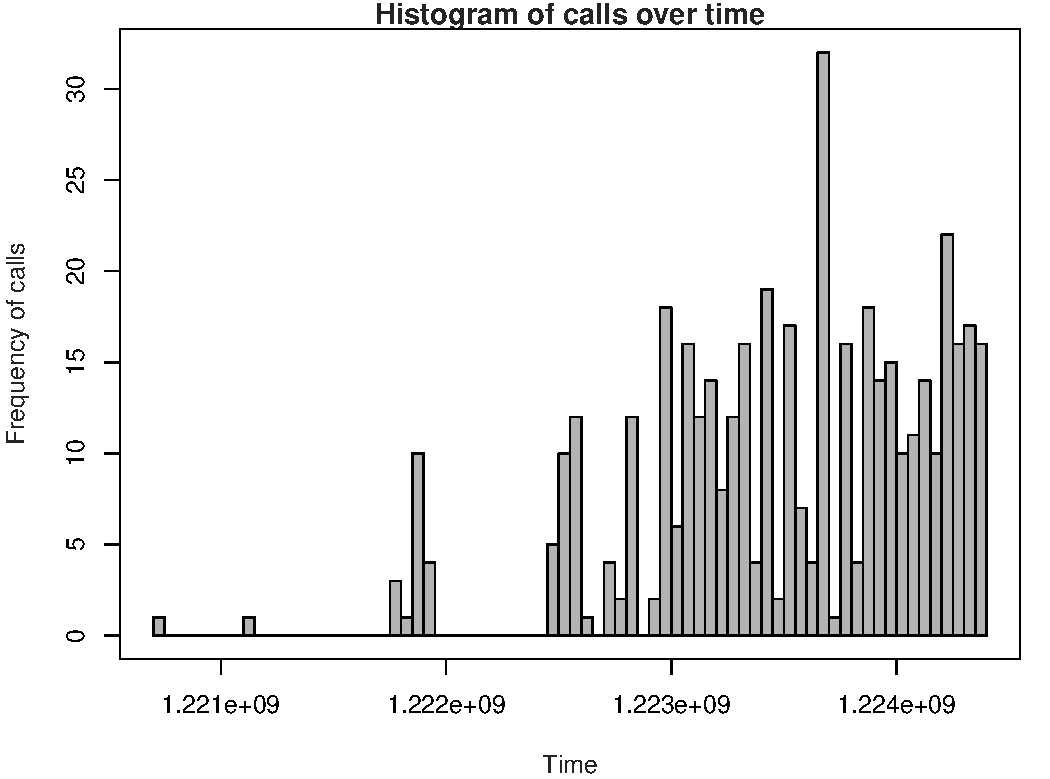
\includegraphics{article-histogram1}
\caption{\label{fig:callstime1} Frequency distribution for number of calls over time.}
\end{figure}
\FloatBarrier



%
%

For simplicity and exhaustivity, the following code examples are run on a small data frame reconstructed from a subset the data \texttt{Social\_Evolution} provided by \pkg{goldfish}. 

% 
% <<subsets>>=
% actors_subset
% calls_subset
% friendship_subset


\subsection[Creating Goldfish objects]{Creating Goldfish objects} \label{subsec:Goldfish_effects}

\subsubsection[Defining the nodeset]{\textbf{Defining the nodeset}} \label{subsubsec:nodeset}


The \texttt{nodes} argument requires a data.frame with information about the nodes that are present throughout the time window of interest. This data.frame must contain at least one vector, which is of the same length as the number of nodes. Other than that it can contain information about the nodes -\texttt{label} (e.g., Actor 1), whether the node is \texttt{present} at the start of the data collection as well as the the initial (at T0), or non-changing values for node attributes. For instance, this data.frame could look like this:

%
\begin{Schunk}
\begin{Soutput}
     label present floor gradeType gender
1  Actor 1    TRUE     4         2      2
2  Actor 2    TRUE     4         2      2
3  Actor 3    TRUE     1         4      2
4  Actor 4    TRUE     8         1      2
5  Actor 5    TRUE     3         1      2
6  Actor 6    TRUE     3         2      2
7  Actor 7    TRUE     4         2      1
8  Actor 8    TRUE     5         5      2
9 Actor 12    TRUE     2         4      2
\end{Soutput}
\end{Schunk}
%

The \texttt{defineNodes} function processes and checks the data.frame passed to \texttt{nodes} argument.
%The nodeset can be defined as such using the following function:
%
\begin{Schunk}
\begin{Sinput}
R> actors <- defineNodes(nodes = actors)  
\end{Sinput}
\end{Schunk}
%


\begin{leftbar}
Please note that \pkg{goldfish} uses the rownames of this data.frame as the internal node IDs. The \texttt{label} variable must be characters.
\end{leftbar}

\newline If you have changing node-attributes you can link \texttt{ChangeEvents} data.frames to the nodeset.  

\newline The \texttt{changeEvents} data.frames mentioned above must be in the following format:
%
\begin{Schunk}
\begin{Soutput}
     time node replace
1 2484870    5   FALSE
2 2487266    5    TRUE
\end{Soutput}
\end{Schunk}
%

Then, \texttt{ChangeEvents} can be linked to the nodeset in the following way:  

%
\begin{Schunk}
\begin{Sinput}
R> actors_ca <- linkEvents(x = actors, 
+                      attribute = "present",
+                      changeEvents = compositionChangeEvents)
\end{Sinput}
\end{Schunk}
%

The \texttt{linkEvents} function links events lists of changing attributes (e.g., present, gender) to the nodeset. The nodeset can be specified with the argument \texttt{x}, the attribute that is changed with the events list has to be defined in the \texttt{attribute} argument as a string. The \texttt{changeEvents} contains a data.frame that describes when and how the nodes attributes change. If no data is linked to an attribute, the attribute variables specified in the \texttt{nodes} arguments are assumed to stay constant (e.g., gender). 

\begin{leftbar}
Note that \texttt{present}, if given as a node attribute, must be true at a given time point for any node to be involved in an event. In the case of a friendship and phone call network with other dynamic actor attributes, someone losing their phone should not be specified as present = false, since then their friendships and individual attributes cannot change. A separate attribute and corresponding event list should be added in such situations that only one type of event cannot occur for a given actor.  
\end{leftbar}

Here the \texttt{time} column in numeric (presented in seconds) or POSIXct format indicates when the change happens. The \texttt{node} column must correspond with either the row number of the nodes data.frame or the label string. The column \texttt{replace} contains boolean values indicating whether the node is present at that time. For instance, the example above shows that node 5 leaves the network at 2484870 seconds but joins back the network at 2487266 seconds. 

It is also possible to link other types of changing attributes in the nodeset, either in numeric or character format (e.g people changing floors). Moreover, in the case of a numeric attribute, we could also add up incremental values to the existing ones by using a column named \texttt{increment} instead of \texttt{replace}

% \newline Other types of node attribute changes (e.g., on which floor an actor lives) are specified with the same data.frame type:
% %
% <<moveEvents, eval=TRUE, echo=FALSE>>=
% moveEvents <- data.frame(time = c(2484800,2484900), node = 7, replace = c(7,5))
% @
% %
% 
% <<moveEventsshow, eval=TRUE, echo=TRUE>>=
% moveEvents
% @
% %
% 
% 
% If the column indicating the change is called \texttt{replace}, \pkg{goldfish} expects values that replace the previous state of the node (e.g., actor 3 moves from floor 3 to floor 5: replace = 5). Alternatively, the increment can be specified (e.g., increment = 2). For this, the column must be named \texttt{increment}. 
% 
% Similarly, \texttt{moveEvents} can be linked to the nodeset:  
% 
% %
% <<linkmoveEvents, eval=TRUE, echo=TRUE>>=
% actors_ca <- linkEvents(x = actors_ca, 
%                     attribute = "floor",
%                     changeEvents = moveEvents)



\subsubsection[Network]{\textbf{Define the network}} \label{subsubsec:networks}


Now that we have defined our nodeset, we want to define a network between the nodes according to an event list.
To do so, a second data.frame is needed, which consists in an edgelist of events happening between actors (e.g tie creations). While the nodes argument must be an object defined with the \texttt{defineNodes} function, the event list should be a data.frame containing the following columns:

%
\begin{Schunk}
\begin{Soutput}
      time  sender receiver increment
1  1936225 Actor 5  Actor 8         1
2  2484877 Actor 7  Actor 4         1
3  2484925 Actor 7  Actor 1         1
4  2485369 Actor 7  Actor 6         1
5  2485377 Actor 6  Actor 7         1
6  2487252 Actor 7  Actor 2         1
7  2522527 Actor 3 Actor 12         1
8  2523087 Actor 3 Actor 12         1
9  2524522 Actor 3 Actor 12         1
10 2524804 Actor 3 Actor 12         1
11 2534595 Actor 3 Actor 12         1
\end{Soutput}
\end{Schunk}
%

As a first step, we define a network object from the nodeset: 
%
\begin{Schunk}
\begin{Sinput}
R> callNetwork <- defineNetwork(nodes = actors_ca, directed = T)
\end{Sinput}
\end{Schunk}
%
 The argument "directed" is \texttt{TRUE} by default, but we need to specify the nodes so that \pkg{goldfish} can check for consistency and relate it to that nodeset as needed.
 

\begin{leftbar}
Note that we have not added any network data yet. By default, defineNetwork() just constructs an empty matrix with dimensions defined by the length of the nodeset(s). So we have an empty network as a starting state.
\end{leftbar}

Now that \pkg{goldfish} recognises the matrix as a network, we can also associate an event list that updates it.
To do this we use the \texttt{linkEvents} function, which requires us to identify a goldfish object to be updated, the events that update it and, in this case, also the nodes that the events should relate to. 
%
\begin{Schunk}
\begin{Sinput}
R> callNetwork <- linkEvents(x = callNetwork, changeEvent = calls_subset, 
+                            nodes = actors_ca)
\end{Sinput}
\end{Schunk}
%


\subsubsection[Define the independent networks]{\textbf{Define the independent networks}} \label{subsubsec:indep_networks}


%
%


Networks that function as independent variables can also be defined with the following function:
%
\begin{Schunk}
\begin{Sinput}
R> friendshipNetwork <- defineNetwork(matrix =friendship.w1, nodes = actors_ca, 
+                                     directed = T)
\end{Sinput}
\end{Schunk}
%



Here the sociomatrix \texttt{friendship.w1} describes the initial state of the network at T0. 

%
%latex.default(friendship.w1, caption = paste("Friendship Sociomatrix Subset"),     file = "", size = "footnotesize", label = paste0("tab:sociomat"),     na.blank = TRUE, longtable = TRUE)%
\setlongtables{\footnotesize
\begin{longtable}{lrrrrrrrrr}\caption{Friendship Sociomatrix Subset} \tabularnewline
\hline\hline
\multicolumn{1}{l}{friendship.w1}&\multicolumn{1}{c}{Actor 1}&\multicolumn{1}{c}{Actor 2}&\multicolumn{1}{c}{Actor 3}&\multicolumn{1}{c}{Actor 4}&\multicolumn{1}{c}{Actor 5}&\multicolumn{1}{c}{Actor 6}&\multicolumn{1}{c}{Actor 7}&\multicolumn{1}{c}{Actor 8}&\multicolumn{1}{c}{Actor 12}\tabularnewline
\hline
\endfirsthead\caption[]{\em (continued)} \tabularnewline
\hline
\multicolumn{1}{l}{friendship.w1}&\multicolumn{1}{c}{Actor 1}&\multicolumn{1}{c}{Actor 2}&\multicolumn{1}{c}{Actor 3}&\multicolumn{1}{c}{Actor 4}&\multicolumn{1}{c}{Actor 5}&\multicolumn{1}{c}{Actor 6}&\multicolumn{1}{c}{Actor 7}&\multicolumn{1}{c}{Actor 8}&\multicolumn{1}{c}{Actor 12}\tabularnewline
\hline
\endhead
\hline
\endfoot
\label{tab:sociomat}
Actor 1&$0$&$0$&$0$&$0$&$0$&$1$&$1$&$0$&$0$\tabularnewline
Actor 2&$0$&$0$&$0$&$0$&$0$&$0$&$0$&$0$&$0$\tabularnewline
Actor 3&$0$&$0$&$0$&$0$&$0$&$0$&$0$&$0$&$1$\tabularnewline
Actor 4&$0$&$0$&$0$&$0$&$0$&$0$&$0$&$0$&$0$\tabularnewline
Actor 5&$0$&$0$&$0$&$0$&$0$&$0$&$0$&$0$&$0$\tabularnewline
Actor 6&$1$&$0$&$0$&$0$&$0$&$0$&$1$&$0$&$0$\tabularnewline
Actor 7&$1$&$1$&$0$&$0$&$0$&$1$&$0$&$0$&$0$\tabularnewline
Actor 8&$0$&$0$&$0$&$0$&$0$&$0$&$0$&$0$&$0$\tabularnewline
Actor 12&$0$&$0$&$1$&$0$&$0$&$0$&$0$&$0$&$0$\tabularnewline
\hline
\end{longtable}}%

\FloatBarrier
\begin{figure}[h!]
\centering
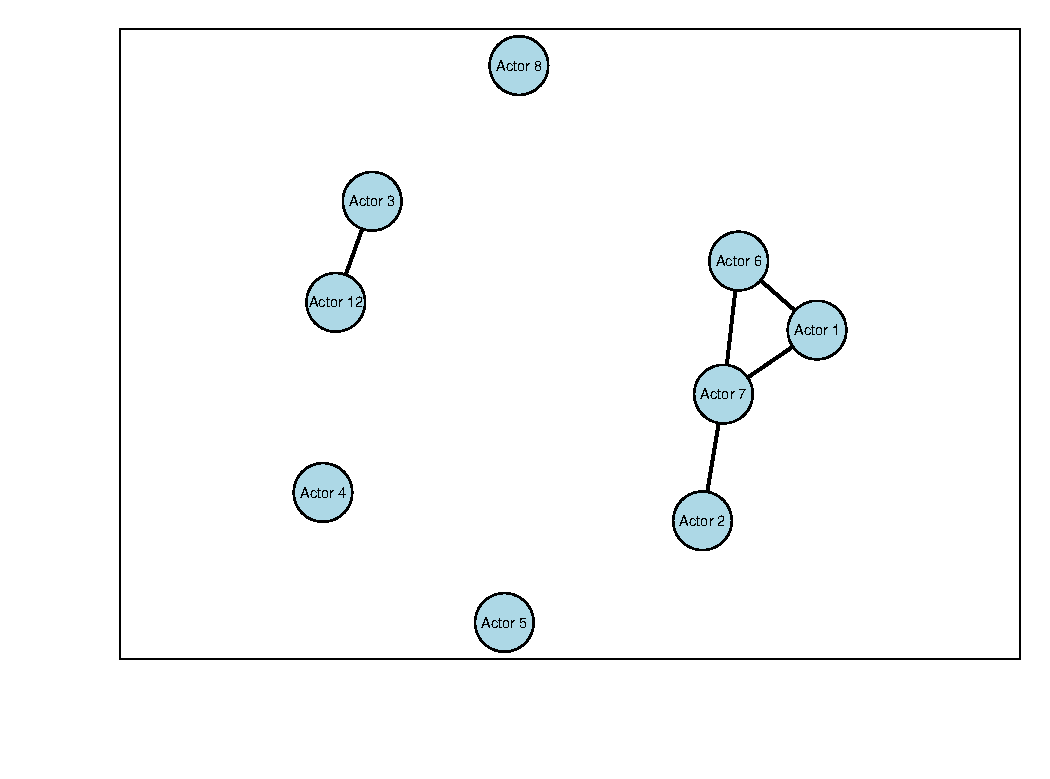
\includegraphics{article-histogram}
\caption{\label{fig:friendnet} Network representation of the Friendship sociomatric subset.}
\end{figure}
\FloatBarrier

This matrix must contain the same nodeset as defined with the \texttt{defineNodes} function and the order of the rows must correspond. The matrix must be binary\textbf{(?)} and can be directed or undirected (as specified with the directed argument). If no matrix is provided, \pkg{goldfish} assumes the initial state to be empty (i.e., a matrix containing only 0s). 

\newline If this network is updated over time (e.g., a new wave of friendship data is collected), these changes can be added with the \texttt{linkEvents} function - similar to link changing attribute events to a nodeset. This time, the user needs to provide the network and the associated nodeset.

The data.frame passed to the \textt{changeEvents} argument must be in the following format:

%
%

%
\begin{Schunk}
\begin{Sinput}
R> friendshipChange
\end{Sinput}
\begin{Soutput}
     time  sender receiver replace
1 4374400 Actor 1  Actor 4       1
2 4374400 Actor 7  Actor 4       1
3 4374400 Actor 6  Actor 1       0
4 4374400 Actor 7  Actor 1       0
\end{Soutput}
\end{Schunk}
%
Then the events can be linked again. 
%
\begin{Schunk}
\begin{Sinput}
R> friendshipNetwork <- linkEvents(x = friendshipNetwork,
+                                  nodes = actors_ca,
+                                  changeEvents = friendshipChange)
\end{Sinput}
\end{Schunk}
%

Alternatively to the \texttt{replace} column, a column called  \texttt{increment} can be used, as we mentioned earlier. For friendship networks, 1 = tie creation, -1 = tie dissolution. The columns  \texttt{sender} and  \texttt{receiver} can be in the format numeric or character. For the numeric case, the entries must correspond to the rownumbers of the nodes data.frame. When character strings are used, they must correspond to the labels in the nodes data.frame. In the example shown above, Actor 4 nominates actor 7 as a friend at timepoint 100 and at timepoint 103 Actor 3 drops the tie to Actor 2.


\subsubsection[Global attributes]{\textbf{Global attributes} \label{subsubsec:glogal_attr}}

Imagine that you want to include a variable that is identical for each node but changes over time. For instance, seasonal climate changes. Such a changing global attribute can be defined with the \texttt{defineGlobalAttribute} function.

%
\begin{Schunk}
\begin{Sinput}
R> seasons <- defineGlobalAttribute(data.frame(time = 1:12, replace = 1:12))
\end{Sinput}
\end{Schunk}
%



\subsubsection[Define the dependent event list]{\textbf{Define the dependent event list}} \label{subsubsec:event_list}

The final step in defining the data objects is to identify the dependent events. Here we would like to model the calls between individuals as the dependent variable using \texttt{calls\_subset}.

While the nodes argument must be an object defined with the \texttt{defineNodes} function, the dependent events defined by \texttt{defineDependentEvents} should take a data.frame as input, containing the following columns: 
%
\begin{Schunk}
\begin{Sinput}
R> callsDependent <- defineDependentEvents(events = calls_subset, 
+                                          nodes = actors_ca, 
+                                          defaultNetwork = callNetwork)
\end{Sinput}
\end{Schunk}
%

\subsubsection[Object visualisation and plot options]{\textbf{Object visualisation and plot options}} \label{subsubsec:plot_options}



\section[Estimation]{Estimation} \label{subsec:estim}
\begin{enumerate}[-]
\item Explanation of the rate and the choice models in the goldfish model 
\item Formulas and mathematical description of each model. 
\item The following code serves as an example and application to the previously explained models. 
\end{enumerate}


In previous section we have defined our dependent network, in the example case this was the call network. The next stage is to specify and fit a model. This step will be performed on the \texttt{Social\_Evolution} dataset. It can be broken up into three steps: the model specification, the preprocessing and the estimation.


The three first steps have been presented in the \hyperref[subsubsec:dep_networks]{previous sections}.
%



\subsection[Model specification]{Step 1: Model specification} \label{subsec:model_specification}

The first step of the estimation procedure consists in specifying our model from the effects and variables available using the standard R formula.

In the case of the rate model, the formula can be specified with attribute effects:
\begin{Schunk}
\begin{Sinput}
R> formula_rate<-(callsDependent ~ alter(actors$gradeType) 
+                 + same(actors$floor))
\end{Sinput}
\end{Schunk}

while in the choice model, we would rather specify the formula with network effects, to which we can add arguments, such as \texttt{window} and \texttt{ignoreRep}.
\begin{Schunk}
\begin{Sinput}
R> formula_choice<-(callsDependent ~ inertia(callNetwork, window=3600) 
+                   + recip(callNetwork, ignoreRep=T) 
+                   + trans(callNetwork, weighted=T))
\end{Sinput}
\end{Schunk}

Beyond the tilde we specify effects and the variables for which the effects are expected to occur. To see the possible effects, use the function \texttt{goldfishEffects}.



\subsection[Step 2: Preprocessing]{Step 2: Preprocessing} \label{subsec:preprocess}

The second step consists of preprocessing which calculates the change statistics associated with the chosen effects.To have a look at the preprocessed objects, we need to activate the \texttt{preprocessingOnly} argument to \texttt{TRUE}:
%
\begin{Schunk}
\begin{Sinput}
R> (DynamM_est_rate<- estimate(formula_rate, model="DyNAM", 
+                              subModel="rate",
+                              preprocessingOnly = T))
\end{Sinput}
\end{Schunk}
%
The same can be done for the choice model simply by replacing \texttt{subModel="rate"} by \texttt{subModel="choice"}.


\subsection[Step 3: Estimation]{Step 3: Estimation} \label{subsec:preprocess}

The third step consists in estimation. The \texttt{estimate} function fit an appropriate model to these statistics.

The rate model can be estimated by specifying the model as \texttt{"DyNAM"} and the submodel as \texttt{"choice"}:

%
\begin{Schunk}
\begin{Sinput}
R> (DynamM_est_rate<- estimate(formula_rate, model="DyNAM", 
+                              subModel="rate"))
\end{Sinput}
\end{Schunk}

%
\begin{Schunk}
\begin{Soutput}
   name               V2         est  std.err sig          t
1 alter actors$gradeType -19.8746576 3.003861 *** -6.6163698
2  same     actors$floor   0.9876948 1.298199      0.7608191
  Log likelihood -1923.3349 
  Converged with max abs. score of 8e-05 
  AIC  3850.66981 
  BIC  3858.83881 
  Model type: DyNAM-M-Rate 
\end{Soutput}
\end{Schunk}


Again, by replacing \texttt{"rate"} by \texttt{"choice"} in the \texttt{subModel} argument, we can obtain the estimation results for the choice model: 

\begin{Schunk}
\begin{Sinput}
R> (DynamM_est_choice<- estimate(formula_choice, model="DyNAM", 
+                                subModel="choice"))
\end{Sinput}
\end{Schunk}


\begin{Schunk}
\begin{Soutput}
     name               V2 ignoreRep weighted window       est
1 inertia callNetwork_3600                      3600 6.2793659
2   recip      callNetwork         B                 2.9821517
3   trans      callNetwork                  W        0.3234464
    std.err sig         t
1 0.2132116 *** 29.451331
2 0.2679389 *** 11.129970
3 0.1924422      1.680745
  Log likelihood -1232.9717 
  Converged with max abs. score of 9e-05 
  AIC  2471.94344 
  BIC  2484.19694 
  Model type: DyNAM-M 
\end{Soutput}
\end{Schunk}

However, in \pkg{goldfish} we also have the option of accelerating this process and using memory more efficiently by combining these three sub-steps in one. Nonetheless, it can be helpful to think of 2a separately, and recognise steps 2b and 2c as \pkg{goldfish} does them.


\subsection[Additional models]{Additional models} \label{subsec:addmodel}

\begin{leftbar}
Note that \pkg{goldfish} provides additionnal models such as the \texttt("coordination") submodel (Stadtfeld, Hollway and Block, 2017) and the \texttt{"REM"} model(Butts, 2008).
\end{leftbar}


% To sum up, provided that we don't have any exogenous changing attributes to add to the nodeset, the simplest full estimation procedure can be run in only 4 steps:
% \begin{enumerate}[1)]
% \item Define the set of nodes as a network object
% \item Link the nodes to the event list in the new network object
% \item Define the dependent events of the network object
% \item Run the estimation procedure.
% \end{enumerate}



\section[Interpreting and diagnosing results]{Interpreting and diagnosing results} \label{subsec:diag_results}

\section[Extending DyNAMs and REMs with own effects]{Extending DyNAMs and REMs with own effects} \label{sec:extensions}

\section[Conclusions]{Conclusions} \label{sec:conclusions}

%% -- Introduction -------------------------------------------------------------

%% - In principle "as usual".
%% - But should typically have some discussion of both _software_ and _methods_.
%% - Use \proglang{}, \pkg{}, and \code{} markup throughout the manuscript.
%% - If such markup is in (sub)section titles, a plain text version has to be
%%   added as well.
%% - All software mentioned should be properly \cite-d.
%% - All abbreviations should be introduced.
%% - Unless the expansions of abbreviations are proper names (like "Journal
%%   of Statistical Software" above) they should be in sentence case (like
%%   "generalized linear models" below).


% For writing about software JSS requires authors to use the markup
% \verb|\proglang{}| (programming languages and large programmable systems),
% \verb|\pkg{}| (software packages), \verb|\code{}| (functions, commands,
% arguments, etc.). If there is such markup in (sub)section titles (as above), a
% plain text version has to be provided in the {\LaTeX} command as well. Below we
% also illustrate how abbrevations should be introduced and citation commands can
% be employed. See the {\LaTeX} code for more details.
% \end{leftbar}
% 
% Modeling count variables is a common task in economics and the social sciences.
% The classical Poisson regression model for count data is often of limited use in
% these disciplines because empirical count data sets typically exhibit
% overdispersion and/or an excess number of zeros. The former issue can be
% addressed by extending  the plain Poisson regression model in various
% directions: e.g., using sandwich covariances or estimating an additional
% dispersion parameter (in a so-called quasi-Poisson model). Another more formal
% way is to use a negative binomial (NB) regression. All of these models belong to
% the family of generalized linear models (GLMs). However, although these models
% typically can capture overdispersion rather well, they are in many applications
% not sufficient for  modeling excess zeros. Since \cite{Mullahy:1986} there is
% increased interest in zero-augmented models that address this issue by a second
% model component capturing zero counts. An overview of count data models in
% econometrics, including  hurdle and zero-inflated models, is provided in
% \cite{Cameron+Trivedi:2013}.
% 
% In \proglang{R} \citep{R}, GLMs are provided by the model fitting functions
% \fct{glm} in the \pkg{stats} package and \fct{glm.nb} in the \pkg{MASS} package
% \citep[][Chapter~7.4]{Venables+Ripley:2002} along with associated methods for
% diagnostics and inference. The manuscript that this document is based on
% \citep{Zeileis+Kleiber+Jackman:2008} then introduced hurdle and zero-inflated
% count models in the functions \fct{hurdle} and \fct{zeroinfl} in the \pkg{pscl}
% package \citep{Jackman:2015}. Of course, much more software could be discussed
% here, including (but not limited to) generalized additive models for count data
% as available in the \proglang{R} packages \pkg{mgcv} \cite{Wood:2006}, 
% \pkg{gamlss} \citep{Stasinopoulos+Rigby:2007}, or \pkg{VGAM} \citep{Yee:2009}.
% 

%% -- Summary/conclusions/discussion -------------------------------------------

\section{Summary and discussion} \label{sec:summary}

\begin{leftbar}
As usual \dots
\end{leftbar}


%% -- Optional special unnumbered sections -------------------------------------

\section*{Computational details}

\begin{leftbar}
If necessary or useful, information about certain computational details
such as version numbers, operating systems, or compilers could be included
in an unnumbered section. Also, auxiliary packages (say, for visualizations,
maps, tables, \dots) that are not cited in the main text can be credited here.
\end{leftbar}

The results in this paper were obtained using
\proglang{R}~3.6.0 with the
\pkg{MASS}~7.3.51.4 package. \proglang{R} itself
and all packages used are available from the Comprehensive
\proglang{R} Archive Network (CRAN) at
\url{https://CRAN.R-project.org/}.

\section*{Acknowledgments}

\begin{leftbar}
All acknowledgments (note the AE spelling) should be collected in this
unnumbered section before the references. It may contain the usual information
about funding and feedback from colleagues/reviewers/etc. Furthermore,
information such as relative contributions of the authors may be added here
(if any).
\end{leftbar}


%% -- Bibliography -------------------------------------------------------------
%% - References need to be provided in a .bib BibTeX database.
%% - All references should be made with \cite, \citet, \citep, \citealp etc.
%%   (and never hard-coded). See the FAQ for details.
%% - JSS-specific markup (\proglang, \pkg, \code) should be used in the .bib.
%% - Titles in the .bib should be in title case.
%% - DOIs should be included where available.

%\bibliography{refs_copie}



\bibliography{literature_goldfish_vignette}

%% -- Appendix (if any) --------------------------------------------------------
%% - After the bibliography with page break.
%% - With proper section titles and _not_ just "Appendix".

\newpage

\begin{appendix}

\section{More technical details} \label{app:technical}

\begin{leftbar}
Appendices can be included after the bibliography (with a page break). Each
section within the appendix should have a proper section title (rather than
just \emph{Appendix}).

For more technical style details, please check out JSS's style FAQ at
\url{https://www.jstatsoft.org/pages/view/style#frequently-asked-questions}
which includes the following topics:
\begin{itemize}
  \item Title vs.\ sentence case.
  \item Graphics formatting.
  \item Naming conventions.
  \item Turning JSS manuscripts into \proglang{R} package vignettes.
  \item Trouble shooting.
  \item Many other potentially helpful details\dots
\end{itemize}
\end{leftbar}


\section[Using BibTeX]{Using \textsc{Bib}{\TeX}} \label{app:bibtex}

\begin{leftbar}
References need to be provided in a \textsc{Bib}{\TeX} file (\code{.bib}). All
references should be made with \verb|\cite|, \verb|\citet|, \verb|\citep|,
\verb|\citealp| etc.\ (and never hard-coded). This commands yield different
formats of author-year citations and allow to include additional details (e.g.,
pages, chapters, \dots) in brackets. In case you are not familiar with these
commands see the JSS style FAQ for details.

Cleaning up \textsc{Bib}{\TeX} files is a somewhat tedious task -- especially
when acquiring the entries automatically from mixed online sources. However,
it is important that informations are complete and presented in a consistent
style to avoid confusions. JSS requires the following format.
\begin{itemize}
  \item JSS-specific markup (\verb|\proglang|, \verb|\pkg|, \verb|\code|) should
    be used in the references.
  \item Titles should be in title case.
  \item Journal titles should not be abbreviated and in title case.
  \item DOIs should be included where available.
  \item Software should be properly cited as well. For \proglang{R} packages
    \code{citation("pkgname")} typically provides a good starting point.
\end{itemize}
\end{leftbar}

\end{appendix}

%% -----------------------------------------------------------------------------


\end{document}
